Table~\ref{tab:comparison} summarizes representative metrics. Figures~\ref{fig:svr} and \ref{fig:evs} illustrate speed retention and energy speed trends.

\begin{table}[!t]
\caption{Representative metrics from literature (indicative order).}
\label{tab:comparison}
\centering
\begin{tabular}{@{}lccccc@{}}
\toprule
Tech. & Speed & Retention & Endurance & Energy/bit & Cell \\
 & ns & s & cycles & fJ & area \\
\midrule
DRAM  & \(\sim 10\) & \(\sim 6.4\times 10^{-2}\) & \(\ge 10^{16}\) & 10--100 & \(6F^{2}\) \\
FeRAM & \(\lesssim 10\) & \(\ge 10^{5}\) & \(10^{12}\)–\(10^{13}\) & \(10^{2}\)–\(10^{3}\) & 1T (FeFET) \\
\bottomrule
\end{tabular}
\end{table}

\begin{figure}[!t]
\centering
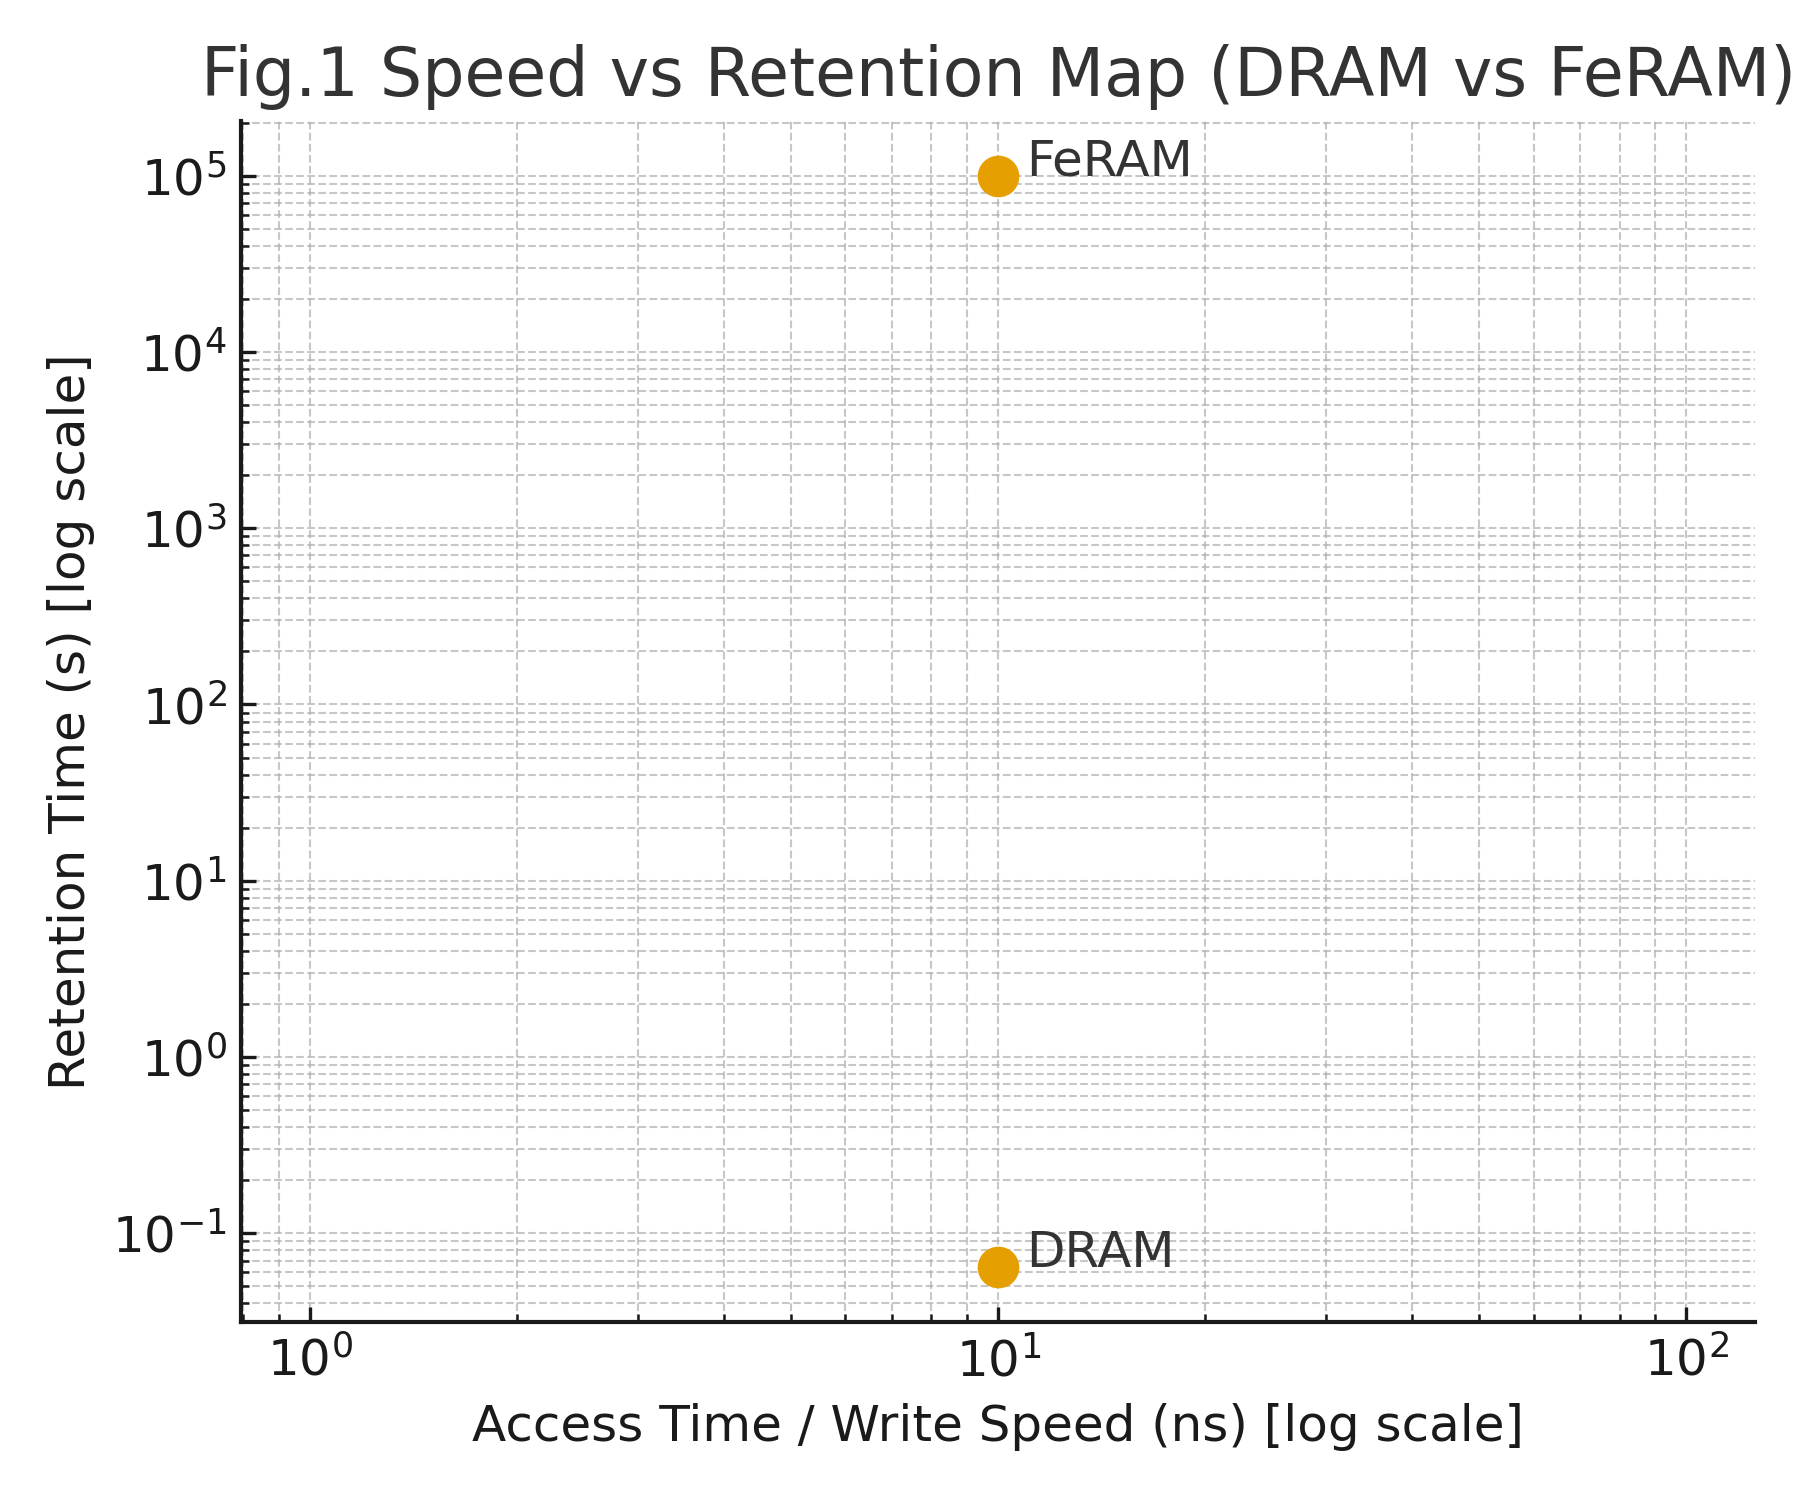
\includegraphics[width=\linewidth]{fig1_speed_vs_retention.png}
\caption{Speed vs retention (illustrative).}
\label{fig:svr}
\end{figure}

\begin{figure}[!t]
\centering
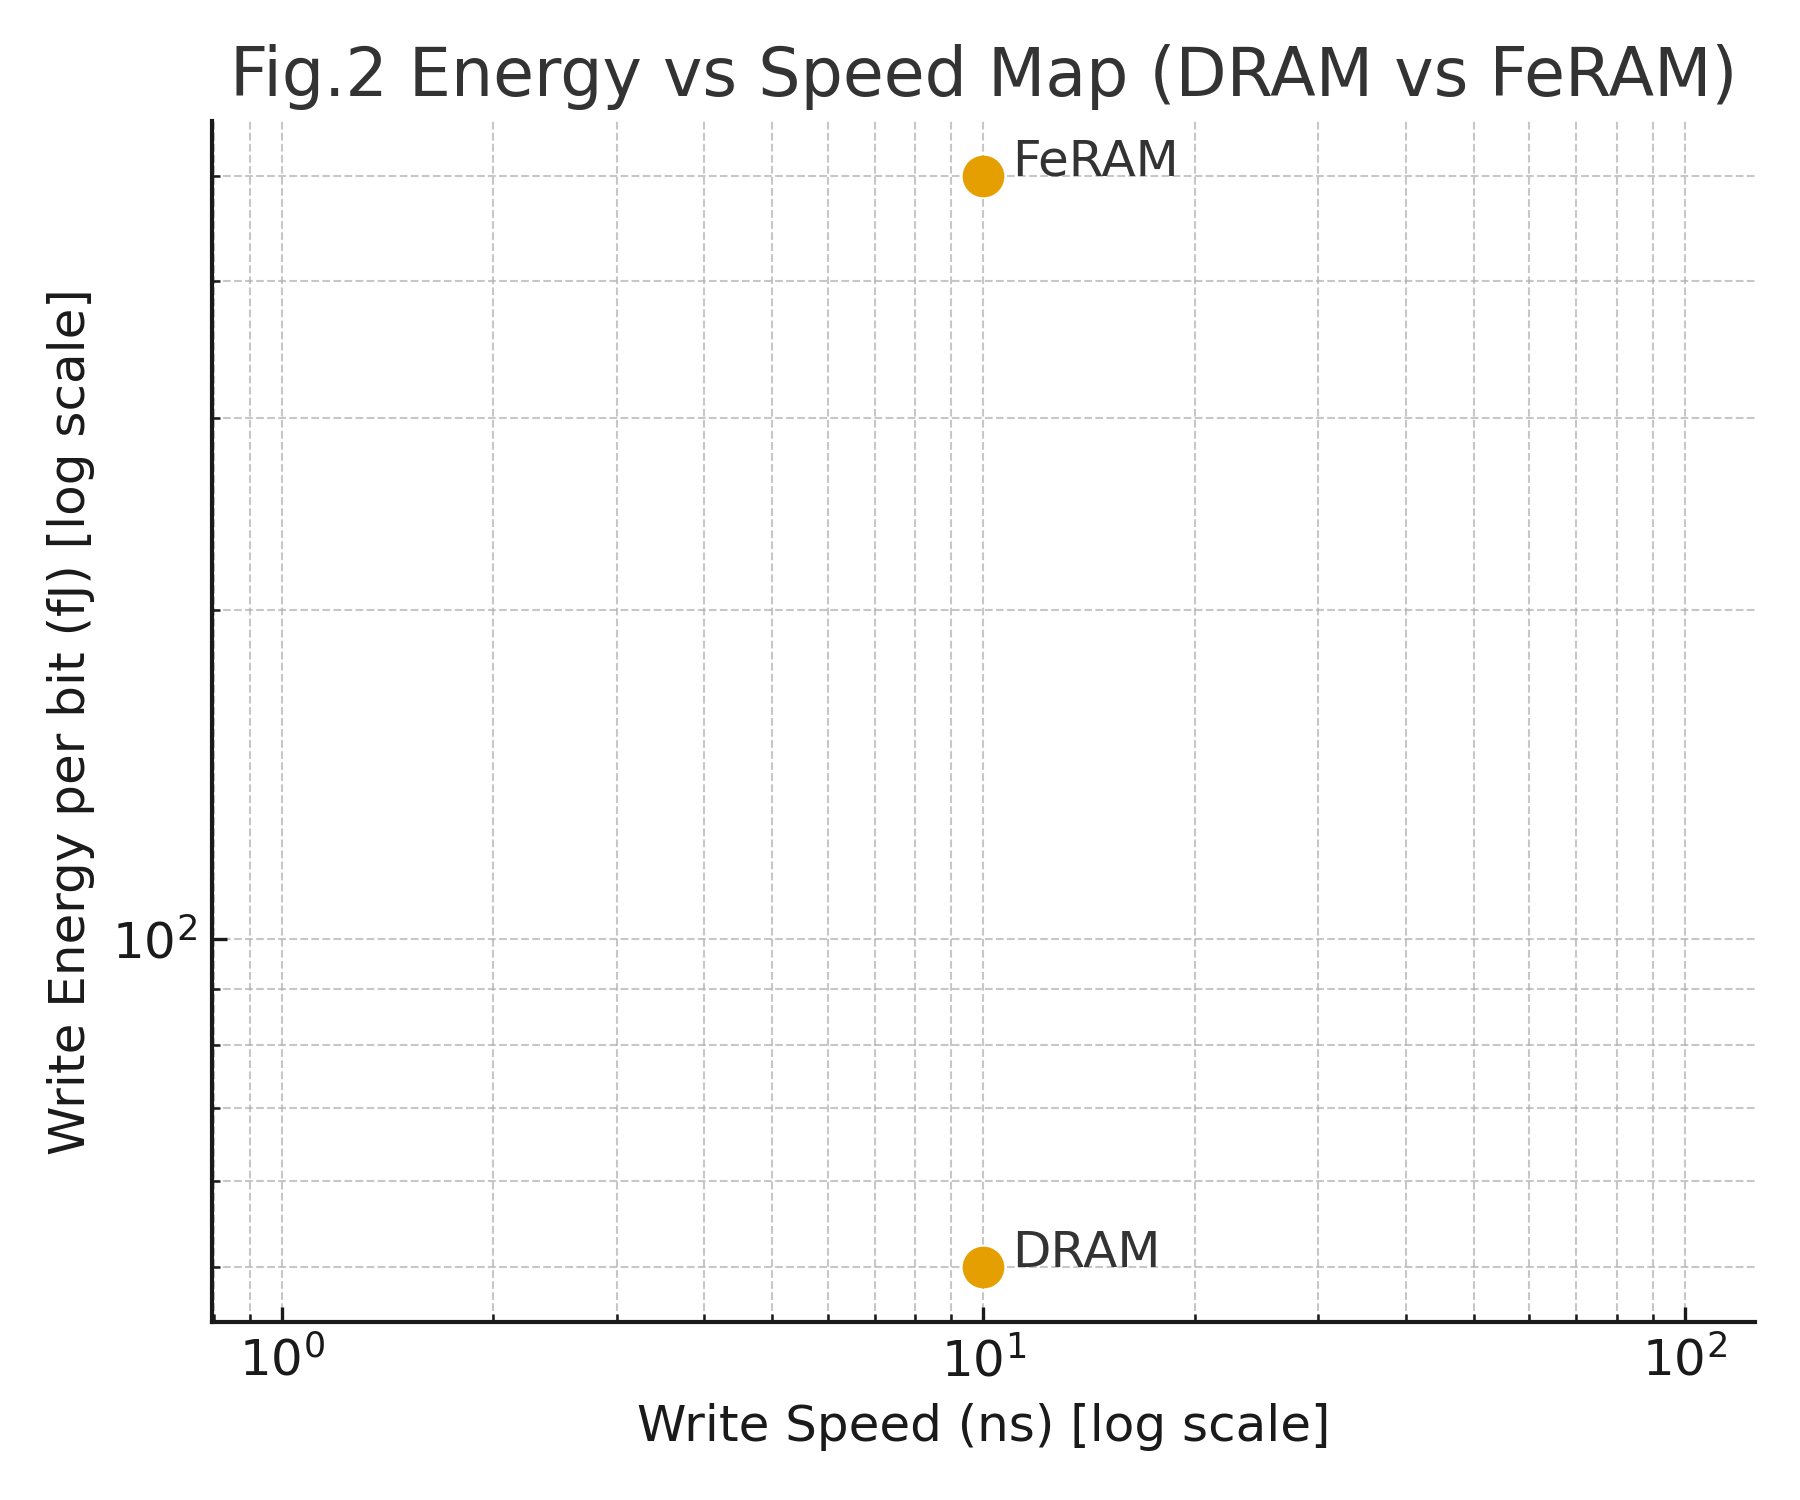
\includegraphics[width=\linewidth]{fig2_energy_vs_speed.png}
\caption{Write energy per bit vs write speed (illustrative).}
\label{fig:evs}
\end{figure}
